
%% bare_conf.tex
%% V1.3
%% 2007/01/11
%% by Michael Shell
%% See:
%% http://www.michaelshell.org/
%% for current contact information.
%%
%% This is a skeleton file demonstrating the use of IEEEtran.cls
%% (requires IEEEtran.cls version 1.7 or later) with an IEEE conference paper.
%%
%% Support sites:
%% http://www.michaelshell.org/tex/ieeetran/
%% http://www.ctan.org/tex-archive/macros/latex/contrib/IEEEtran/
%% and
%% http://www.ieee.org/

%%*************************************************************************
%% Legal Notice:
%% This code is offered as-is without any warranty either expressed or
%% implied; without even the implied warranty of MERCHANTABILITY or
%% FITNESS FOR A PARTICULAR PURPOSE! 
%% User assumes all risk.
%% In no event shall IEEE or any contributor to this code be liable for
%% any damages or losses, including, but not limited to, incidental,
%% consequential, or any other damages, resulting from the use or misuse
%% of any information contained here.
%%
%% All comments are the opinions of their respective authors and are not
%% necessarily endorsed by the IEEE.
%%
%% This work is distributed under the LaTeX Project Public License (LPPL)
%% ( http://www.latex-project.org/ ) version 1.3, and may be freely used,
%% distributed and modified. A copy of the LPPL, version 1.3, is included
%% in the base LaTeX documentation of all distributions of LaTeX released
%% 2003/12/01 or later.
%% Retain all contribution notices and credits.
%% ** Modified files should be clearly indicated as such, including  **
%% ** renaming them and changing author support contact information. **
%%
%% File list of work: IEEEtran.cls, IEEEtran_HOWTO.pdf, bare_adv.tex,
%%                    bare_conf.tex, bare_jrnl.tex, bare_jrnl_compsoc.tex
%%*************************************************************************

% *** Authors should verify (and, if needed, correct) their LaTeX system  ***
% *** with the testflow diagnostic prior to trusting their LaTeX platform ***
% *** with production work. IEEE's font choices can trigger bugs that do  ***
% *** not appear when using other class files.                            ***
% The testflow support page is at:
% http://www.michaelshell.org/tex/testflow/



% Note that the a4paper option is mainly intended so that authors in
% countries using A4 can easily print to A4 and see how their papers will
% look in print - the typesetting of the document will not typically be
% affected with changes in paper size (but the bottom and side margins will).
% Use the testflow package mentioned above to verify correct handling of
% both paper sizes by the user's LaTeX system.
%
% Also note that the "draftcls" or "draftclsnofoot", not "draft", option
% should be used if it is desired that the figures are to be displayed in
% draft mode.
%
\documentclass[conference]{IEEEtran}
% Add the compsoc option for Computer Society conferences.
%
% If IEEEtran.cls has not been installed into the LaTeX system files,
% manually specify the path to it like:
% \documentclass[conference]{../sty/IEEEtran}

% The following packages can be found on http:\\www.ctan.org
\usepackage{graphics} % for pdf, bitmapped graphics files
\usepackage{epsfig} % for postscript graphics files
\usepackage{mathptmx} % assumes new font selection scheme installed
\usepackage{times} % assumes new font selection scheme installed
\usepackage{amsmath} % assumes amsmath package installed
\usepackage{amssymb}  % assumes amsmath package installed
\usepackage{lipsum,amsmath,multicol}
\usepackage{tikz}
\usetikzlibrary{fit,positioning}

%\usepackage[numbers]{natbib}
\usepackage{multicol}
\usepackage[bookmarks=true]{hyperref}

%\usepackage{caption}
%%\usepackage{subfigure}
%\usepackage{wrapfig}
%\usepackage{placeins}
%\usepackage{graphicx}
%\usepackage{amssymb,amsmath}
\usepackage[position=bottom,labelfont=bf,textfont={sl,bf},lofdepth,lotdepth]{subfig}



% Some very useful LaTeX packages include:
% (uncomment the ones you want to load)


% *** MISC UTILITY PACKAGES ***
%
%\usepackage{ifpdf}
% Heiko Oberdiek's ifpdf.sty is very useful if you need conditional
% compilation based on whether the output is pdf or dvi.
% usage:
% \ifpdf
%   % pdf code
% \else
%   % dvi code
% \fi
% The latest version of ifpdf.sty can be obtained from:
% http://www.ctan.org/tex-archive/macros/latex/contrib/oberdiek/
% Also, note that IEEEtran.cls V1.7 and later provides a builtin
% \ifCLASSINFOpdf conditional that works the same way.
% When switching from latex to pdflatex and vice-versa, the compiler may
% have to be run twice to clear warning/error messages.






% *** CITATION PACKAGES ***
%
%\usepackage{cite}
% cite.sty was written by Donald Arseneau
% V1.6 and later of IEEEtran pre-defines the format of the cite.sty package
% \cite{} output to follow that of IEEE. Loading the cite package will
% result in citation numbers being automatically sorted and properly
% "compressed/ranged". e.g., [1], [9], [2], [7], [5], [6] without using
% cite.sty will become [1], [2], [5]--[7], [9] using cite.sty. cite.sty's
% \cite will automatically add leading space, if needed. Use cite.sty's
% noadjust option (cite.sty V3.8 and later) if you want to turn this off.
% cite.sty is already installed on most LaTeX systems. Be sure and use
% version 4.0 (2003-05-27) and later if using hyperref.sty. cite.sty does
% not currently provide for hyperlinked citations.
% The latest version can be obtained at:
% http://www.ctan.org/tex-archive/macros/latex/contrib/cite/
% The documentation is contained in the cite.sty file itself.






% *** GRAPHICS RELATED PACKAGES ***
%
\ifCLASSINFOpdf
  % \usepackage[pdftex]{graphicx}
  % declare the path(s) where your graphic files are
  % \graphicspath{{../pdf/}{../jpeg/}}
  % and their extensions so you won't have to specify these with
  % every instance of \includegraphics
  % \DeclareGraphicsExtensions{.pdf,.jpeg,.png}
\else
  % or other class option (dvipsone, dvipdf, if not using dvips). graphicx
  % will default to the driver specified in the system graphics.cfg if no
  % driver is specified.
  % \usepackage[dvips]{graphicx}
  % declare the path(s) where your graphic files are
  % \graphicspath{{../eps/}}
  % and their extensions so you won't have to specify these with
  % every instance of \includegraphics
  % \DeclareGraphicsExtensions{.eps}
\fi
% graphicx was written by David Carlisle and Sebastian Rahtz. It is
% required if you want graphics, photos, etc. graphicx.sty is already
% installed on most LaTeX systems. The latest version and documentation can
% be obtained at: 
% http://www.ctan.org/tex-archive/macros/latex/required/graphics/
% Another good source of documentation is "Using Imported Graphics in
% LaTeX2e" by Keith Reckdahl which can be found as epslatex.ps or
% epslatex.pdf at: http://www.ctan.org/tex-archive/info/
%
% latex, and pdflatex in dvi mode, support graphics in encapsulated
% postscript (.eps) format. pdflatex in pdf mode supports graphics
% in .pdf, .jpeg, .png and .mps (metapost) formats. Users should ensure
% that all non-photo figures use a vector format (.eps, .pdf, .mps) and
% not a bitmapped formats (.jpeg, .png). IEEE frowns on bitmapped formats
% which can result in "jaggedy"/blurry rendering of lines and letters as
% well as large increases in file sizes.
%
% You can find documentation about the pdfTeX application at:
% http://www.tug.org/applications/pdftex





% *** MATH PACKAGES ***
%
%\usepackage[cmex10]{amsmath}
% A popular package from the American Mathematical Society that provides
% many useful and powerful commands for dealing with mathematics. If using
% it, be sure to load this package with the cmex10 option to ensure that
% only type 1 fonts will utilized at all point sizes. Without this option,
% it is possible that some math symbols, particularly those within
% footnotes, will be rendered in bitmap form which will result in a
% document that can not be IEEE Xplore compliant!
%
% Also, note that the amsmath package sets \interdisplaylinepenalty to 10000
% thus preventing page breaks from occurring within multiline equations. Use:
%\interdisplaylinepenalty=2500
% after loading amsmath to restore such page breaks as IEEEtran.cls normally
% does. amsmath.sty is already installed on most LaTeX systems. The latest
% version and documentation can be obtained at:
% http://www.ctan.org/tex-archive/macros/latex/required/amslatex/math/





% *** SPECIALIZED LIST PACKAGES ***
%
%\usepackage{algorithmic}
% algorithmic.sty was written by Peter Williams and Rogerio Brito.
% This package provides an algorithmic environment fo describing algorithms.
% You can use the algorithmic environment in-text or within a figure
% environment to provide for a floating algorithm. Do NOT use the algorithm
% floating environment provided by algorithm.sty (by the same authors) or
% algorithm2e.sty (by Christophe Fiorio) as IEEE does not use dedicated
% algorithm float types and packages that provide these will not provide
% correct IEEE style captions. The latest version and documentation of
% algorithmic.sty can be obtained at:
% http://www.ctan.org/tex-archive/macros/latex/contrib/algorithms/
% There is also a support site at:
% http://algorithms.berlios.de/index.html
% Also of interest may be the (relatively newer and more customizable)
% algorithmicx.sty package by Szasz Janos:
% http://www.ctan.org/tex-archive/macros/latex/contrib/algorithmicx/




% *** ALIGNMENT PACKAGES ***
%
%\usepackage{array}
% Frank Mittelbach's and David Carlisle's array.sty patches and improves
% the standard LaTeX2e array and tabular environments to provide better
% appearance and additional user controls. As the default LaTeX2e table
% generation code is lacking to the point of almost being broken with
% respect to the quality of the end results, all users are strongly
% advised to use an enhanced (at the very least that provided by array.sty)
% set of table tools. array.sty is already installed on most systems. The
% latest version and documentation can be obtained at:
% http://www.ctan.org/tex-archive/macros/latex/required/tools/


%\usepackage{mdwmath}
%\usepackage{mdwtab}
% Also highly recommended is Mark Wooding's extremely powerful MDW tools,
% especially mdwmath.sty and mdwtab.sty which are used to format equations
% and tables, respectively. The MDWtools set is already installed on most
% LaTeX systems. The lastest version and documentation is available at:
% http://www.ctan.org/tex-archive/macros/latex/contrib/mdwtools/


% IEEEtran contains the IEEEeqnarray family of commands that can be used to
% generate multiline equations as well as matrices, tables, etc., of high
% quality.


%\usepackage{eqparbox}
% Also of notable interest is Scott Pakin's eqparbox package for creating
% (automatically sized) equal width boxes - aka "natural width parboxes".
% Available at:
% http://www.ctan.org/tex-archive/macros/latex/contrib/eqparbox/





% *** SUBFIGURE PACKAGES ***
%\usepackage[tight,footnotesize]{subfigure}
% subfigure.sty was written by Steven Douglas Cochran. This package makes it
% easy to put subfigures in your figures. e.g., "Figure 1a and 1b". For IEEE
% work, it is a good idea to load it with the tight package option to reduce
% the amount of white space around the subfigures. subfigure.sty is already
% installed on most LaTeX systems. The latest version and documentation can
% be obtained at:
% http://www.ctan.org/tex-archive/obsolete/macros/latex/contrib/subfigure/
% subfigure.sty has been superceeded by subfig.sty.



%\usepackage[caption=false]{caption}
%\usepackage[font=footnotesize]{subfig}
% subfig.sty, also written by Steven Douglas Cochran, is the modern
% replacement for subfigure.sty. However, subfig.sty requires and
% automatically loads Axel Sommerfeldt's caption.sty which will override
% IEEEtran.cls handling of captions and this will result in nonIEEE style
% figure/table captions. To prevent this problem, be sure and preload
% caption.sty with its "caption=false" package option. This is will preserve
% IEEEtran.cls handing of captions. Version 1.3 (2005/06/28) and later 
% (recommended due to many improvements over 1.2) of subfig.sty supports
% the caption=false option directly:
%\usepackage[caption=false,font=footnotesize]{subfig}
%
% The latest version and documentation can be obtained at:
% http://www.ctan.org/tex-archive/macros/latex/contrib/subfig/
% The latest version and documentation of caption.sty can be obtained at:
% http://www.ctan.org/tex-archive/macros/latex/contrib/caption/




% *** FLOAT PACKAGES ***
%
%\usepackage{fixltx2e}
% fixltx2e, the successor to the earlier fix2col.sty, was written by
% Frank Mittelbach and David Carlisle. This package corrects a few problems
% in the LaTeX2e kernel, the most notable of which is that in current
% LaTeX2e releases, the ordering of single and double column floats is not
% guaranteed to be preserved. Thus, an unpatched LaTeX2e can allow a
% single column figure to be placed prior to an earlier double column
% figure. The latest version and documentation can be found at:
% http://www.ctan.org/tex-archive/macros/latex/base/



%\usepackage{stfloats}
% stfloats.sty was written by Sigitas Tolusis. This package gives LaTeX2e
% the ability to do double column floats at the bottom of the page as well
% as the top. (e.g., "\begin{figure*}[!b]" is not normally possible in
% LaTeX2e). It also provides a command:
%\fnbelowfloat
% to enable the placement of footnotes below bottom floats (the standard
% LaTeX2e kernel puts them above bottom floats). This is an invasive package
% which rewrites many portions of the LaTeX2e float routines. It may not work
% with other packages that modify the LaTeX2e float routines. The latest
% version and documentation can be obtained at:
% http://www.ctan.org/tex-archive/macros/latex/contrib/sttools/
% Documentation is contained in the stfloats.sty comments as well as in the
% presfull.pdf file. Do not use the stfloats baselinefloat ability as IEEE
% does not allow \baselineskip to stretch. Authors submitting work to the
% IEEE should note that IEEE rarely uses double column equations and
% that authors should try to avoid such use. Do not be tempted to use the
% cuted.sty or midfloat.sty packages (also by Sigitas Tolusis) as IEEE does
% not format its papers in such ways.





% *** PDF, URL AND HYPERLINK PACKAGES ***
%
%\usepackage{url}
% url.sty was written by Donald Arseneau. It provides better support for
% handling and breaking URLs. url.sty is already installed on most LaTeX
% systems. The latest version can be obtained at:
% http://www.ctan.org/tex-archive/macros/latex/contrib/misc/
% Read the url.sty source comments for usage information. Basically,
% \url{my_url_here}.





% *** Do not adjust lengths that control margins, column widths, etc. ***
% *** Do not use packages that alter fonts (such as pslatex).         ***
% There should be no need to do such things with IEEEtran.cls V1.6 and later.
% (Unless specifically asked to do so by the journal or conference you plan
% to submit to, of course. )


% correct bad hyphenation here
\hyphenation{op-tical net-works semi-conduc-tor}


\begin{document}
%
% paper title
% can use linebreaks \\ within to get better formatting as desired
\title{Articulation Estimation Using Depth Sensing}


% author names and affiliations
% use a multiple column layout for up to three different
% affiliations
\author{\IEEEauthorblockN{Suren Kumar }
\IEEEauthorblockA{Mechanical and Aerospace Engineering\\
State University of New York at Buffalo\\
Buffalo, NY, USA\\
Email: surenkum@buffalo.edu}
\and
\IEEEauthorblockN{Vikas Dhiman}
\IEEEauthorblockA{Electrical Engineering\\
University of Michigan \\
 Ann Arbor, MI, USA\\
Email: dhiman@umich.edu }
}


% conference papers do not typically use \thanks and this command
% is locked out in conference mode. If really needed, such as for
% the acknowledgment of grants, issue a \IEEEoverridecommandlockouts
% after \documentclass

% for over three affiliations, or if they all won't fit within the width
% of the page, use this alternative format:
% 
%\author{\IEEEauthorblockN{Michael Shell\IEEEauthorrefmark{1},
%Homer Simpson\IEEEauthorrefmark{2},
%James Kirk\IEEEauthorrefmark{3}, 
%Montgomery Scott\IEEEauthorrefmark{3} and
%Eldon Tyrell\IEEEauthorrefmark{4}}
%\IEEEauthorblockA{\IEEEauthorrefmark{1}School of Electrical and Computer Engineering\\
%Georgia Institute of Technology,
%Atlanta, Georgia 30332--0250\\ Email: see http://www.michaelshell.org/contact.html}
%\IEEEauthorblockA{\IEEEauthorrefmark{2}Twentieth Century Fox, Springfield, USA\\
%Email: homer@thesimpsons.com}
%\IEEEauthorblockA{\IEEEauthorrefmark{3}Starfleet Academy, San Francisco, California 96678-2391\\
%Telephone: (800) 555--1212, Fax: (888) 555--1212}
%\IEEEauthorblockA{\IEEEauthorrefmark{4}Tyrell Inc., 123 Replicant Street, Los Angeles, California 90210--4321}}




% use for special paper notices
%\IEEEspecialpapernotice{(Invited Paper)}




% make the title area
\maketitle

\IEEEpeerreviewmaketitle
\begin{abstract}
\begin{itemize}
  \item Detect distinctly moving clustered points/voxels/objects in a scene.
    \begin{itemize}
      \item Use Kinect fusion to create a static map.
      \item Use some kind of noise threshold to detect object movement
        independent of camera movement.
      \item Trigger algorithm (may be use RANSAC ?? etc.) that will segment out
        the object that just moved. The object should be spatially clustered
        and should be explained by the same rigid 3D motion. 
      \item Maintain a pairwise relative localization graph of the scene.
    \end{itemize}
  \item Semantic reasoning in map update of these objects and their
    localization.  Reason about Physical support and articulated linkage.
  \item Build a 3D reconstruction of these objects.
  \item Find similar unmapped static objects in the scene. May be use Jeff's
    detection and segmentation code.
  \item Try algorithm for long term mapping (~ a week) by using auto charging
    turtlebots in a living room and compare with existing algorithms.
\end{itemize}
\end{abstract}
% IEEEtran.cls defaults to using nonbold math in the Abstract.
% This preserves the distinction between vectors and scalars. However,
% if the conference you are submitting to favors bold math in the abstract,
% then you can use LaTeX's standard command \boldmath at the very start
% of the abstract to achieve this. Many IEEE journals/conferences frown on
% math in the abstract anyway.

% no keywords

\section{Introduction}
Imagine a robot moving in a typical living room environment which encounters indoor objects such as doors, drawers and chairs etc. We posit that in order for the robot to understand, map or interact with such objects, the robot needs to be able to understand the articulation. Pyschophysical experiments on human motion understanding have demonstrated that human first distinguish between competing motion models (translation, rotation and expansion) and then estimate the motion conditioned on motion model \cite{NIPS2008_3458}.

\section{Related Work}

\subsection{Historical Perspective}
Using image motion to understand motion and structure in the scene is a historically well studied problem in computer vision.  Ullman \cite{ullman1979interpretation} proposed that in non-degenerate cases under orthographic projection, three pictures of four points can determine structure and motion. Tomasi and Kanade \cite{tomasi1992shape} formalized Ullmans's idea and proposed one of the influential method to compute camera motion and image structure by tracking features in the images. They proposed factorizing a matrix of feature tracks into motion and shape matrix by enforcing the rank constraint of the rigid body motion and metric constraints of a rotation matrix. Costeira and Kanade \cite{costeira1998multibody} extended the factorization idea to segment and recover shape along with motion of multiple moving bodies in the scene. 

Yan and Pollefeys \cite{yan2006automatic} further extended this rank and subspace idea to estimate kinematic chains from tracked features. There are certain fundamental limitations which is common to these approaches. First, the reliance on feature tracking methods such as KLT is not suitable for indoor environments which may not have much texture. Furthermore, this feature tracking requirement limits the application of such methods tremendously by i) Not being able to track new parts/objects that enter/exit the scene, ii) Not modelling the entire scene and as a result not exploring dependencies between neighbouring objects, iii) Restricting the ability to assimilate the motion of objects in SLAM like approaches that map the entire scene. Secondly, motion orthogonal to image plane is not modelled \cite{yan2006automatic} as image projection is modelled as affine projection in the most general case. 

With the discovery of cheap and commonplace hardware such as Kinect, there is a need to re-examine this structure from motion idea. First, since such hardware already provides depth for a feature point, one already has shape as estimated by traditional structure from motion. Also since depth is available, one can model the motion orthogonal to image plane. Texture-less objects can be tracked by adding depth edges to the tracking mix.


\cite{martin2014online} Build on existing work on articulation estimation. Add interactive perception where manipulation adds to perception and vice versa.
  \cite{yan2006automatic} 
    Problem: Analysis and reconstruction of dynamical scenes
    Method: Estimate the rigid motion subspaces. Extend the method to non-rigid
    parts by modeling it with linear combination of key shapes. Use motion
    segmentation ( by SVD) to segment feature trajectories for each object. Use
    n neighbors to estimate local subspace of each point and cluster the
    subspaces to estimate the cluster of trajectories that form the same metric subspace.

    \cite{katz2010interactive} uses RGB for 3D articulation estimation.
    \cite{katz2013interactive} Uses RGBD

 
TODO: Anguelov et al. - kinematic models of doors
TODO: Yan and Pollefeys : Assumes affine geometry. Only revolute joints.


TODO: \cite{sturm20103d} : 3D trajectories by manipulation of environment \\
TODO: \cite{huang2012occlusion} \\ 
TODO: \cite{Pillai-RSS-14} \\


\section{Articulation Classification}\label{sec:articulation_classification} We consider the problem of motion model identification from point correspondences of motion. In the current work, we consider revolute, prismatic and general motion. Consider motion of two points $x_0,x_1$ (represented in an inertial frame) on a rigid body at time $t_0$ and at some subsequent times $t_1,t_2$. The most general form of rigid body motion of a point can be represented using a rotation matrix $R$ and an associated translation vector $T$
\begin{align}
x_0^{t_1}& = R_{t_0}^{t_1}x_0^{t_0}+T_{t_0}^{t_1}
\end{align}
where the superscript on the point denotes the time.
\subsection{Prismatic}
For points lying on a prismatic joint such as a drawer, rotation w.r.t inertial frame remains the same (R=I), resulting in $x_1^{t_1}-x_0^{t_1} = x_1^{t_0}-x_0^{t_0}$. This is essentially saying that the vector joining two points on a prismatic joint remains the same before and after the motion.
\subsection{Revolute}
For further distinction between revolute and general motion, we need information from more than one time step. For points lying on a body undergoing revolute motion such as a door, the points have same translation vector over time. Hence estimating the translation vector from two time steps $T_{t_0}^{t_1} = T_{t_1}^{t_2}$ is a sufficient condition to classify a joint as revolute joint. 
\subsection{Plane Constrained Motion} Plane constrained motion is useful for characterizing motion of objects like chair that can be translated on a plane and rotated about the normal to the plane. Let the plane be denoted by an point $x_p$ lying on the plane and $\hat{n}$ being normal to that plane. Consider the case of a rigid body that has point $x_c^{t_0}$ in contact with the ground plane which after undergoing the motion moves to $x_c^{t_1}$. Since $x_c^{t_0}$ and $x_c^{t_1}$ both lie on the ground plane, we have
\begin{align}
(x_c^{t_0}-x_0)^T\hat{n}&=0\\
(x_c^{t_1}-x_0)^T\hat{n}&=0\\
x_c^{t_1} &= R_{t_0}^{t_1}x_c^{t_0}+T_{t_0}^{t_1}
\end{align}
By doing algebraic manipulation we get, $(R_{t_0}^{t_1}x_0+T-x_0)^T\hat{n}=0$

\subsection{General Rigid Body Motion}
For general motion such as a book that can be rotated and translated anywhere in the space both the rotation and translation matrix will be different. 
\section{Scene Understanding}
Analysis by method such as ours is essential in order to decompose the scene into types of motion that a robot can influence on the scene.
For example: Understanding the way a drawer can be opened, fridge door can be opened, what can be moved around in the scene

Other important use cases of motion estimation
\begin{itemize}
\item Estimation a joint can induce prior over objects such as revolute joint can induce prior over refrigerator and door
\item Visual object identification such as drawer can induce a prior over motion estimation
\item Object tracking 
\item For grasping? -- such as how to open a door?
\end{itemize}

\section{Factorization Approach} In this section, we extend the factorization approach as described in \cite{costeira1998multibody} to 3-D track data available from a depth camera. Assuming for now that a single object moves relative to a static camera and we track features from frame to frame. Following the notation in the paper, lets represent a point on the object as $p_i^T = [X_i,Y_i,Z_i]^T$ in the camera frame, in the current frame $f$, the position of the point in homogeneous coordinates can be represented as 
\begin{align}
s_{fi}^C = \begin{bmatrix} 
p_{fi}^C\\1
\end{bmatrix}
&=\begin{bmatrix}
R_f & t_f\\
0_{1\times3}& 1
\end{bmatrix}
\begin{bmatrix}
p_i\\
1
\end{bmatrix}
= \begin{bmatrix}
R_f & t_f\\
0_{1\times3}& 1
\end{bmatrix}
s_i
\end{align}
where $R_f$ and $t_f$ are the rotation and translation of the object from current frame w.r.t to the frame in which object points are initially represented. Assuming that we track $N$ features over $F$ frames, one can write 
\begin{align}
\begin{bmatrix}
u_{11} & ... & u_{1N} \\ 
. &  & .\\
u_{F1} & ... & u_{FN} \\ 
v_{11} & ... & v_{1N} \\ 
. &  & .\\
v_{F1} & ... & v_{FN} \\ 
w_{11} & ... & w_{1N} \\ 
. &  & .\\
w_{F1} & ... & w_{FN} \\ 
\end{bmatrix} & = 
\begin{bmatrix}
i_1^T & | & t_{x_1}\\
. & | & .\\
i_F^T & | & t_{x_F}\\
j_1^T & | & t_{y_1}\\
. & | & .\\
j_F^T & | & t_{y_F}\\
k_1^T & | & t_{z_1}\\
. & | & .\\
k_F^T & | & t_{z_F}\\
\end{bmatrix}
\begin{bmatrix}
s_1 & . & . &. & s_N
\end{bmatrix}\label{eq:global_motion}
\end{align}
where $(u_{fi},v_{fi},w_{fi})$ is the location of feature point in current frame, vectors $i_f^T,j_f^T,k_f^T$ are the rows of the rotation matrix $R_f$ and $(t_{x_f},t_{y_f},t_{z_f})$ represent the components of the translation vector at time instant with frame $f$. Equation \ref{eq:global_motion} can be represented in a accumulated form as 
\begin{align}
\mathbf{W} & = \mathbf{M}\mathbf{S}
\end{align}
where $\mathbf{W}$ represents the accumulation from trajectories of $N$ points tracked over $F$ frames, $\mathbf{M}$ contains all the information about the motion of the object present in the scene and $\mathbf{S}$ contains all the information about the shape of the object. Since rank of product of two matrices can not exceed the minimum of rank of individual matrics, It is clear that the maximum rank of $W$ is 4. Computing singular value decomposition of $\mathbf{W}$, we get 
\begin{align}
\mathbf{W} = \mathbf{U}\Sigma\mathbf{V}^T \label{eq:motion_factor}
\end{align}
where $U \in R^{3F \times 4}$, and $V \in R^{N \times 4}$ are left and right real singular matrices and $\Sigma$ is a $4\times4$ diagonal matrix of singular values. Although if $\mathbf{W}$ was full rank, we would have to consider $N$ singular values but as the rank of $W$ is 4, we only write out the components corresponding to first $4$ singular values. Writing the factorization as product of two matrices,
\begin{align}
\mathbf{\hat{M}} = \mathbf{U}\Sigma^{\frac{1}{2}}, \mathbf{\hat{S}} = \Sigma^{\frac{1}{2}}\mathbf{V}^T \label{eq:motion_factor}
\end{align}

\subsection{Motion and Shape Estimation} The factorization as defined in Equation \ref{eq:motion_factor} is not unique as any invertible $4 \times 4$ matrix $A$  will lead to an alternate solution $\mathbf{M} = \mathbf{\hat{M}}A$,  $\mathbf{S} = A^{-1}\mathbf{\hat{S}}$


%\begin{align*}
%a =1
%\end{align*}
%\begin{multicols}{2}
%\lipsum[1-3]
%\end{multicols}
%\par\noindent\rule{\dimexpr(0.5\textwidth-0.5\columnsep-0.4pt)}{0.4pt}%
%\rule{0.4pt}{6pt}
\begin{tiny}
  

\begin{equation}
\begin{bmatrix}
m_{00}^2 & 2m_{00}m_{01} & 2m_{00}m_{02} & m_{01}^2 & 2m_{01}m_{02} & m_{02}^2 \\
 m_{10}m_{00} & m_{10}m_{01}+ m_{11}m_{00}  & m_{10}m_{02} + m_{12}m_{00}& m_{11}m_{01} & m_{11}m_{02}  + m_{12}m_{01} & m_{12}m_{02}\\
 m_{20}m_{00} &  m_{20}m_{01}+ m_{21}m_{00 }&   m_{20}m_{02} + m_{22}m_{00} &  m_{21}m_{01} & m_{21}m_{02} + m_{22}m_{01} & m_{22}m_{02}\\
m_{00}m_{10} & m_{00}m_{11} + m_{01}m_{10} & m_{00}m_{12} + m_{02}m_{10} & m_{01}m_{11} & m_{01}m_{12} + m_{02}m_{11} & m_{02}m_{12}\\
 m_{10}^2 & 2m_{10}m_{11} & 2m_{10}m_{12} &  m_{11}^2 & 2m_{11}m_{12} & m_{12}^2\\
 m_{20}m_{10} & m_{20}m_{11}+ m_{21}m_{10} &  m_{20}m_{12}+ m_{22}m_{10} &  m_{21}m_{11}& m_{21}m_{12} + m_{22}m_{11} & m_{22}m_{12}\\
 m_{00}m_{20} & m_{00}m_{21} + m_{01}m_{20} & m_{00}m_{22} + m_{02}m_{20} & m_{01}m_{21} & m_{01}m_{22} + m_{02}m_{21} & m_{02}m_{22}\\
m_{10}m_{20} & m_{10}m_{21} + m_{11}m_{20} & m_{10}m_{22} + m_{12}m_{20} & m_{11}m_{21} & m_{11}m_{22} + m_{12}m_{21} & m_{12}m_{22}\\
 m_{20}^2 & 2m_{20}m_{21}& 2m_{20}m_{22} & m_{21}^2 & 2m_{21}m_{22} & m_{22}^2
 
\end{bmatrix} \\
\begin{bmatrix}
a_{00}\\
a_{01}\\
a_{02}\\
a_{11}\\
a_{12}\\
a_{22}
\end{bmatrix} = 
\begin{bmatrix}
1\\
0\\
0\\
0\\
1\\
0\\
0\\
0\\
1
\end{bmatrix}
\label{eq:least_sq_aat}
\end{equation}

\end{tiny}


%\begin{equation}
%\begin{bmatrix}
%m_{11}^2 & 2m_{11}m_{12} & 2m_{11}m_{13} & 2m_{11}m_{14}& m_{12}^2&2m_{12}m_{13}&2m_{12}m_{14}&m_{13}^2&2m_{13}m_{14}&m_{14}^2 \\
% m_{21}m_{11} & m_{21}m_{12}+m_{22}m_{11}  & m_{21}m_{13}+ m_{23}m_{11}&m_{21}m_{14}+m_{24}m_{11} & m_{22} m_{12}& m_{22}m_{13}+m_{23}m_{12}& m_{22}m_{14} +m_{24} m_{12} & m_{23}m_{13}  & m_{23}m_{14}+m_{24}m_{13} &m_{24}m_{14}\\
% m_{11}m_{31}& m_{11}m_{32} + m_{12}m_{31} & m_{13}m_{31}+m_{11}m_{33} &  m_{14}m_{31}+ m_{11}m_{34} &  m_{12}m_{32}  &  m_{13}m_{32}+ m_{12}m_{33}&  m_{14}m_{32} + m_{12}m_{34}& m_{13}m_{33} & m_{14}m_{33}+m_{13}m_{34} & m_{14}m_{34}\\
%m_{21}m_{11} & m_{22}m_{11}+m_{21}m_{12} & m_{23}m_{11}+m_{21}m_{13} & m_{24}m_{11}+m_{21}m_{14}&  m_{22}m_{12} &m_{23}m_{12}+ m_{22}m_{13} & m_{24}m_{12}+m_{22}m_{14}& m_{23}m_{13} & m_{24}m_{13}+m_{23}m_{14} & m_{24}m_{14}\\
% m_{21}^2 & 2m_{21}m_{22} & 2m_{21}m_{23} & 2m_{21}m_{24} & m_{22}^2 & 2m_{22}m_{23} &2m_{22}m_{24} & m_{23}^2 & 2m_{23}m_{24} &m_{24}^2\\
%m_{21}m_{31} & m_{22}m_{31}+ m_{21}m_{32} & m_{23}m_{31}+m_{21}m_{33} & m_{24}m_{31}+ m_{21}m_{34} & m_{22}m_{32} & m_{23}m_{32}+ m_{22}m_{33}& m_{24}m_{32} + m_{22}m_{34}&  m_{23}m_{33} & m_{24}m_{33} +m_{23}m_{34} &m_{24}m_{34}\\
% m_{31}m_{11} & m_{32}m_{11} + m_{31}m_{12} & m_{33}m_{11}+m_{31}m_{13} & m_{34}m_{11} + m_{31}m_{14}  & m_{32}m_{12} & m_{33}m_{12}+ m_{32}m_{13}& m_{34}m_{12} + m_{32}m_{14} &  m_{33}m_{13} & m_{34}m_{13}  + m_{33}m_{14} & m_{34}m_{14}\\
%m_{31}m_{21} & m_{32}m_{21} + m_{31}m_{22} & m_{33}m_{21} +m_{31}m_{23} & m_{34}m_{21}+ m_{31}m_{24 } & m_{32}m_{22}& m_{33}m_{22}+ m_{32}m_{23} & m_{34}m_{22}+ m_{32}m_{24} & m_{33}m_{23}& m_{34}m_{23}  + m_{33}m_{24} & m_{34}m_{24}\\
% m_{31}^2 & 2m_{31}m_{32}& 2m_{31}m_{33} & 2m_{31}m_{34} & m_{32}^2 & 2m_{32}m_{33} & 2m_{32}m_{34} & m_{33}^2 & 2m_{33}m_{34} & m_{34}^2]
% 
%\end{bmatrix} \\
%\begin{bmatrix}
%a_{11}\\
%a_{12}\\
%a_{13}\\
%a_{14}\\
%a_{22}\\
%a_{23}\\
%a_{24}\\
%a_{33}\\
%a_{34}\\
%a_{44}
%\end{bmatrix} = 
%\begin{bmatrix}
%1\\
%0\\
%0\\
%0\\
%1\\
%0\\
%0\\
%0\\
%1
%\end{bmatrix}
%\label{eq:least_sq_aat}
%\end{equation}

%\vspace{\belowdisplayskip}\hfill\rule[-6pt]{0.4pt}{6.4pt}%
%\rule{\dimexpr(0.5\textwidth-0.5\columnsep-1pt)}{0.4pt}
%\begin{multicols}{2}
%\lipsum[4-5]
%\end{multicols}

\section{SLAM for Dynamic World}
\begin{figure}
\centering
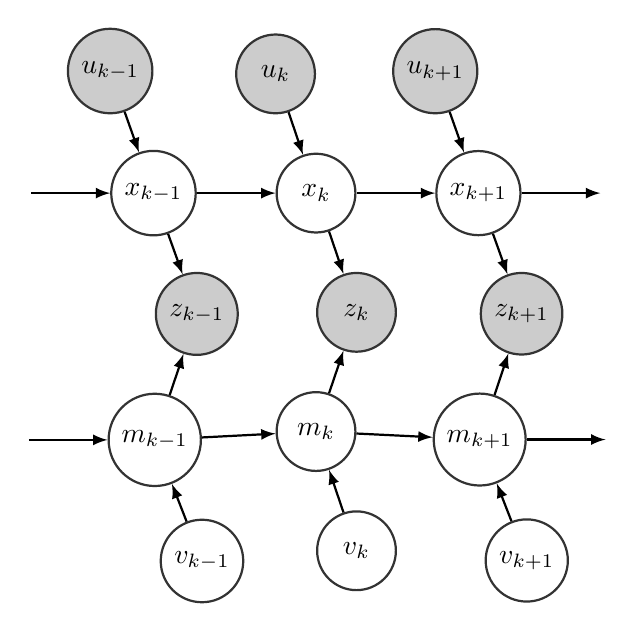
\begin{tikzpicture}
\tikzstyle{main}=[circle, minimum size = 10mm, thick, draw =black!80, node distance = 10mm]
\tikzstyle{connect}=[-latex, thick]
\tikzstyle{box}=[rectangle, draw=black!100]
\coordinate (org_1) at (0,0);
  \node[main] (x_k_1)[right=of org_1] {$x_{k-1}$ };
  \node[main] (x_k) [right=of x_k_1] { $x_{k}$ };
  \node[main] (x_k_2) [right=of x_k] {$x_{k+1}$};
\coordinate[right=of x_k_2] (end_1);

  \node[main, fill = black!20] (u_k_1)[above=of x_k_1.west] {$u_{k-1}$ };
\node[main, fill = black!20] (u_k)[above=of x_k.west] {$u_{k}$ };
\node[main, fill = black!20] (u_k_2)[above=of x_k_2.west] {$u_{k+1}$ };

\node[main, fill = black!20] (z_k_1)[below=of x_k_1.east] {$z_{k-1}$ };
\node[main, fill = black!20] (z_k)[below=of x_k.east] {$z_{k}$ };
\node[main, fill = black!20] (z_k_2)[below=of x_k_2.east] {$z_{k+1}$ };


\node[main] (m_k_1)[below=of z_k_1.west] {$m_{k-1}$ };
\coordinate [left=of m_k_1](org_2);
\node[main] (m_k)[below=of z_k.west] {$m_{k}$ };
\node[main] (m_k_2)[below=of z_k_2.west] {$m_{k+1}$ };
\coordinate [right=of m_k_2](end_2);

\node[main] (v_k_1)[below=of m_k_1.east] {$v_{k-1}$ };
\node[main] (v_k)[below=of m_k.east] {$v_{k}$ };
\node[main] (v_k_2)[below=of m_k_2.east] {$v_{k+1}$ };


  \path 
 (org_1) edge [connect] (x_k_1)
(x_k_1) edge [connect] (x_k)
(x_k) edge [connect] (x_k_2)
(x_k_2) edge [connect] (end_1)

(u_k_1) edge [connect] (x_k_1)
(u_k) edge [connect] (x_k)
(u_k_2) edge [connect] (x_k_2)

(x_k_1) edge [connect] (z_k_1)
(x_k) edge [connect] (z_k)
(x_k_2) edge [connect] (z_k_2)

(m_k_1) edge [connect] (z_k_1)
(m_k) edge [connect] (z_k)
(m_k_2) edge [connect] (z_k_2)


 (org_2) edge [connect] (m_k_1)
(m_k_1) edge [connect] (m_k)
(m_k) edge [connect] (m_k_2)
(m_k_2) edge [connect] (end_2)

(v_k_1) edge [connect] (m_k_1)
(v_k) edge [connect] (m_k)
(v_k_2) edge [connect] (m_k_2);
\end{tikzpicture}
\caption{Graphical Model of the general SLAM problem. The known nodes are darker than the unknown nodes.}
\label{fig:graphical_model}
\end{figure}
Figure \ref{fig:graphical_model} shows the graphical model of the most general SLAM problem, where $x_k$, $u_k$, $z_k$, $m_k$, $v_k$ represents the robot state, input to the robot, observation by robot, state of the world and action of various agents in the environment.

Basic SLAM algorithms \textit{assume the map $m_{k-1} \equiv m_k \equiv m$ to be static} and model the combination of robot state and map $x_k,m$ as the state of the estimation problem. The estimation problem only requires motion model $P(x_k|x_{k-1},u_k)$ and observation model $P(z_k|x_k,m)$. The observation model assumes the observations to be conditionally independent given the the map and the current vehicle state. The goal of the estimation process is to produce unbiased and consistent estimates (expectation of mean squared error should match filter-calculated covariance) \cite{yaakov2001estimation}.

For the current SLAM problem, the state consists of time-varying map, (unknown input to the world by various agents) and the robot state. Hence the full estimation problem can be posed as 
\begin{align}
P(x_k,m_k|\mathbf{Z}_{0:k},\mathbf{U}_{0:k},\mathbf{V}_{0:k},x_0,m_0)
\end{align}
Following the notation in the review paper on SLAM by Durrant-Whyte and Bailey \cite{durrant2006simultaneous}, $\mathbf{Z}_{0:k}$, $\mathbf{U}_{0:k}$ and $\mathbf{V}_{0:k}$ represent the set of observations, robot control inputs and map control inputs from the start time to time step $k$. It is assumed that the map is markovian in nature which implies that the start state of the map $m_0$ has all the information needed to make future prediction if actions of various agents in the world $v_{k-1},...,v_{k+1}$ and its impact on the map is known.

\subsection{Time update} The time update models the evolution of state according to the motion model. To write equation concisely, let $A =\{ \mathbf{Z}_{0:k-1},\mathbf{U}_{0:k},\mathbf{V}_{0:k},x_0,m_0 \}$
\begin{align}
&P(x_k,m_k|A) = \nonumber \\
&\int \int P(x_k,x_{k-1},m_k,m_{k-1}|A) dx_{k-1} dm_{k-1} \nonumber \\
&\int \int P(x_k|x_{k-1},m_k,m_{k-1},A)P(x_{k-1},m_k,m_{k-1}|A) dx_{k-1}dm_{k-1} \nonumber \\
&\int \int P(x_k|x_{k-1},u_k)P(x_{k-1},m_k,m_{k-1}|A) dx_{k-1}dm_{k-1} \nonumber \\
&\int \int P(x_k|x_{k-1},u_k)P(m_k|x_{k-1},m_{k-1},A)P(x_{k-1},m_{k-1}|A)  dx_{k-1}dm_{k-1} \nonumber \\
&\int \int P(x_k|x_{k-1},u_k)P(m_k|m_{k-1},v_{k-1})P(x_{k-1},m_{k-1}|A) dx_{k-1}dm_{k-1} \nonumber \\
\label{eq:time_update}
\end{align}

The independence relationship in derivation of time update in Equation \ref{eq:time_update} are due to the Bayesian networks in Figure \ref{fig:graphical_model} in which each node is independent of its non-descendants given the parents of that node. Given the structure of time update, we need two motion models, one for robot: $P(x_k|x_{k-1},u_k)$ and another one for the world $P(m_k|m_{k-1},v_{k-1})$. It can be clearly observed that $P(m_k|m_{k-1},v_{k-1})$ for a static map is dirac delta function and integrates out in Equation \ref{eq:time_update}. 

\subsection{Measurement Update} Measurement update uses the bayes formula to update the state of the estimation problem given a new observation $z_k$ at time step $k$. To write the equations concisely, let $B =\{ \mathbf{Z}_{0:k},\mathbf{U}_{0:k},\mathbf{V}_{0:k},x_0,m_0 \}$
 \begin{align}
P(x_k,m_k|B) &= \frac{P(z_k|x_k,m_k,A)P(x_k,m_k|A)}{P(z_k|A)} \nonumber\\
&=\frac{P(z_k|x_k,m_k)P(x_k,m_k|A)}{P(z_k|A)}
\label{eq:measurement_update}
\end{align}

Equation \ref{eq:measurement_update} together with equation \ref{eq:time_update} defines the complete recursive form of the SLAM algorithm for a dynamic environment. Robot motion model and observation model $P(z_k|x_k,m_k)$ are well described in previous literature and hence we will exclude that from current discussion. The focus of current work is the representation of map motion model to extend the standard SLAM algorithm with its static world assumption to dynamic world.

\section{Dynamic World Representation} Real world is dynamic in nature with varying degree of motion such as parking lot which can be assumed to be temporary stationary compared to a road which is always in motion. Previous literature to handle dynamic environments can be divided into two predominant approaches A) Detect moving objects and ignore them, B) Track moving objects as landmarks  \cite{bailey2006simultaneous}. In the first approach, using the fact that the conventional SLAM map is highly redundant, the moving landmarks can be removed from the map building process \cite{bailey2002mobile}. In contrast, Wang et. al \cite{wang2003online} explicitly track moving objects by adding them to the estimation state. However the work assumed that the sensor measurement can be decomposed into observation corresponding to moving and static landmarks which requires good estimate of moving and static landmarks to start with. Furthermore, it was assumed that the measurement of moving object carries no information for the SLAM state estimation implying that the map remains unchanged. A simple counter example is the case of a moving door in an indoor environment which changes the map of the scene.

\subsection{Known Decomposition of the World} Object SLAM+ Object Tracking Interacting multiple models

In feature based mapping, motion of each feature can be assumed to be independent given the location of the feature at previous time step. In dense mapping, a scene/map be decomposed into $n$ different parts such as chair, door etc. whose shape is known. The parts of the scene $m_k = \{b^i_k\},  1\leq i \leq n$ are assumed to move independently and hence the motion of the map can be represented as collection of independent motion of the parts. The true motion model for the  each part of the scene is assumed to be one of the motion models $C \in \{C_j\}^{p}_{j=1}$ as represented in Section \ref{sec:articulation_classification}. 

Dropping the notation for scene part, In current formulation, we assume a uniform prior $\mu_j(0) = P(C_j), \sum_{j=1}^{p}\mu_j(0) = 1$ over different motion models for each scene part. However, this prior can be modified appropriately by object detection such as doors are more likely to have revolute joints etc.. Motion model probability is updated as more and more observations are received \cite{yaakov2001estimation} as 
\begin{align}
& \mu_j(k) \equiv P(C_j|\mathbf{Z}_{0:k})  = 
\frac{P(z_k|\mathbf{Z}_{0:k-1}, C_j)P(C_j|\mathbf{Z}_{0:k-1})}{P(z_k|\mathbf{Z}_{0:k-1})} \nonumber \\
&\mu_j(k) = \frac{P(z_k|\mathbf{Z}_{0:k-1}, C_j)\mu_j(k-1)}{\sum_{j=1}^{p} P(z_k|\mathbf{Z}_{0:k-1}, C_j)\mu_j(k-1) }
\end{align}
The probability of the current observation $z_k$ at time step $k$, conditioned over a specific motion model and all the previous observation can be represented by various method. In the current work, we filter the states using Extended Kalman Filter, for which this probability is the probability of observation residual w.r.t a normal distribution distributed with zero mean and innovation covariance \cite{yaakov2001estimation}.
\subsection{No Prior Information}

\section{Results}
\begin{figure*}
  \usetikzlibrary{calc}
   \begin{tikzpicture}[imgstyle/.style={draw,thick,anchor=south west,inner sep=1pt}]
 %\path[use as bounding box, draw] (0,-1) rectangle (\imgwidth, 0.34\imgwidth);
\node[imgstyle] (img1) at (0,0) {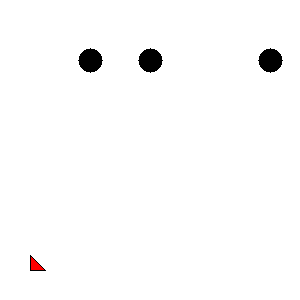
\includegraphics[width=0.32\imgwidth]{media/frame0000.png}};
\node[imgstyle] (img2) at (0.333\imgwidth,0) {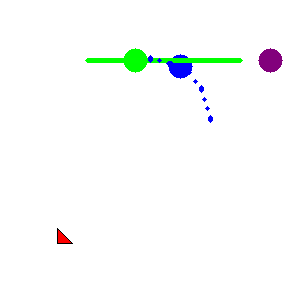
\includegraphics[width=0.32\imgwidth]
{media/frame0003.png}};
\node[imgstyle] (img3) at (0.666\imgwidth,0) {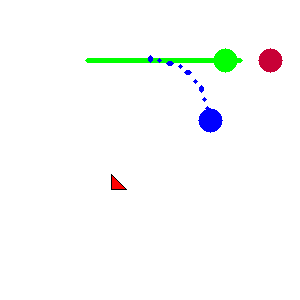
\includegraphics[width=0.32\imgwidth]{media/frame0009.png}};
\begin{scope}[x={(img1.south east)}, y={(img1.north west)}]
\node (r) at (0.3, 0.1) {Robot};
\node (lmks) at (0.7, 0.6) {Landmarks};
\end{scope}
\path ($(img1.south) + (-0.5, -0.5)$) node (ld) {Legend:};
\path 
(ld)
 ++ (1.8, 0) node [circle,fill=green] {} + (1, 0) node {Prismatic}
 ++ (3, 0) node [circle,fill=blue] {} + (1, 0) node {Revolute}
 ++ (3, 0) node [circle,fill=red] {} + (0.8, 0) node {Static}
;

 \end{tikzpicture}

\end{figure*}

\bibliographystyle{unsrt}
\bibliography{articulation_estimation}

% that's all folks
\end{document}


